\texttt{make}はビルトイン型(\texttt{map}、\texttt{slice}および\texttt{channel})のメモリの割り当てです。\texttt{new}は各型のメモリを割り当てます。

ビルトイン関数\texttt{new}は本質的には他の言語で使われる同名の関数と機能が同じです:\texttt{new(T)}はゼロサプレスされた\texttt{T}型のメモリ空間を割り当て、そのアドレスを返します。すなわち\texttt{*T}型の値です。Goの専門用語で言えば、ポインタを返すということです。新たに割り当てられた型\texttt{T}のゼロ値です。とても重要なことに:

\begin{quote}
\texttt{new}はポインタを返します。
\end{quote}

ビルトイン関数\texttt{make(T, args)}と\texttt{new(T)}は異なる機能を持っています。makeは\texttt{slice}、\texttt{map}または\texttt{channel}を作成し、初期値(非ゼロ値)を持つ\texttt{T}型を返すのみで、\texttt{*T}ではありません。本質的には、この3つの型が異なる点はデータ構造を指し示す参照が使用される前に初期化されているということです。例えば、データ(内部\texttt{array})を指し示すポインタ、長さ,容量による3点で記述される\texttt{slice}の各項目が初期化される前は、\texttt{slice}は\texttt{nil}です。\texttt{slice}, \texttt{map}, \texttt{channel}にとって、makeは内部のデータ構造を初期化し、適当な値で埋め尽くされます。


\begin{quote}
\texttt{make}は初期化後の(非ゼロの)値を返します。
\end{quote}




\begin{figure}[H]
  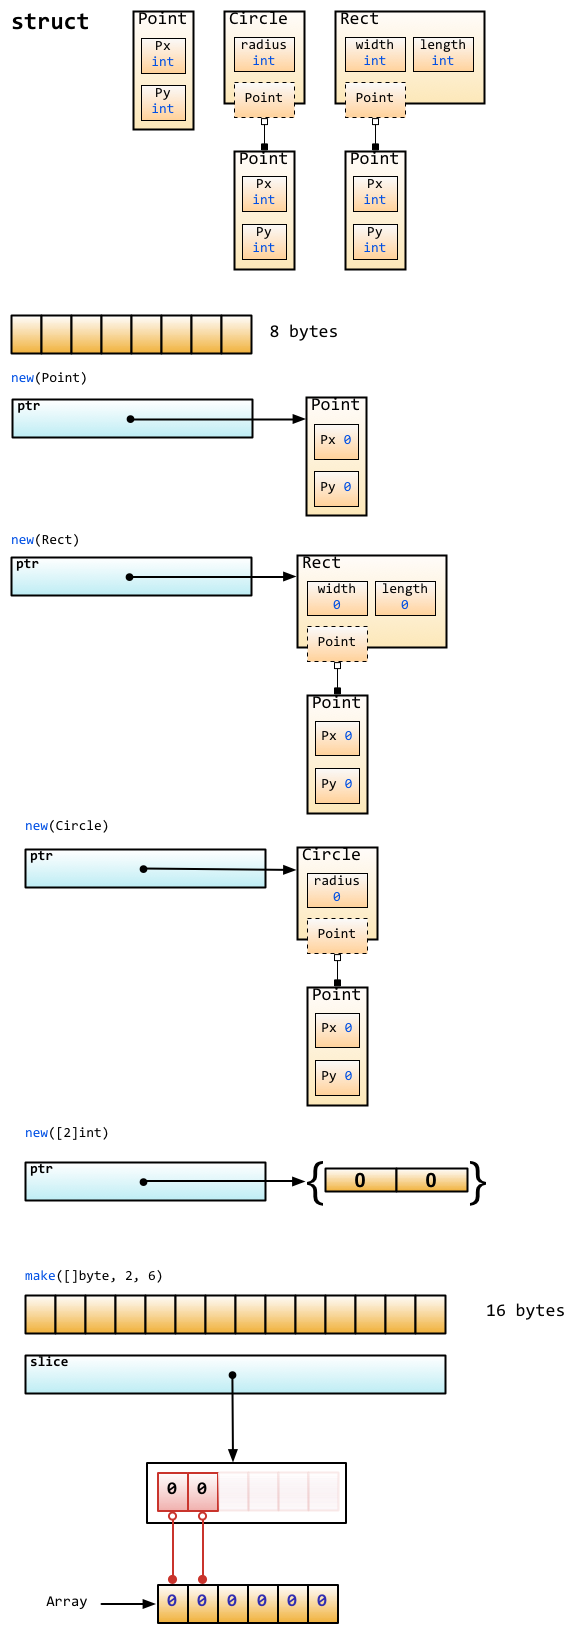
\includegraphics[width=7cm]{2.2.makenew.png}
   \label{図2.5}
   \caption{makeとnewの低レイヤでのメモリの割り当て}
\end{figure}
